% Template for Cogsci submission with R Markdown

% Stuff changed from original Markdown PLOS Template
\documentclass[10pt, letterpaper]{article}

\usepackage{cogsci}
\usepackage{pslatex}
\usepackage{float}
\usepackage{caption}

% amsmath package, useful for mathematical formulas
\usepackage{amsmath}

% amssymb package, useful for mathematical symbols
\usepackage{amssymb}

% hyperref package, useful for hyperlinks
\usepackage{hyperref}

% graphicx package, useful for including eps and pdf graphics
% include graphics with the command \includegraphics
\usepackage{graphicx}

% Sweave(-like)
\usepackage{fancyvrb}
\DefineVerbatimEnvironment{Sinput}{Verbatim}{fontshape=sl}
\DefineVerbatimEnvironment{Soutput}{Verbatim}{}
\DefineVerbatimEnvironment{Scode}{Verbatim}{fontshape=sl}
\newenvironment{Schunk}{}{}
\DefineVerbatimEnvironment{Code}{Verbatim}{}
\DefineVerbatimEnvironment{CodeInput}{Verbatim}{fontshape=sl}
\DefineVerbatimEnvironment{CodeOutput}{Verbatim}{}
\newenvironment{CodeChunk}{}{}

% cite package, to clean up citations in the main text. Do not remove.
\usepackage{cite}

\usepackage{color}

% Use doublespacing - comment out for single spacing
%\usepackage{setspace}
%\doublespacing


% % Text layout
% \topmargin 0.0cm
% \oddsidemargin 0.5cm
% \evensidemargin 0.5cm
% \textwidth 16cm
% \textheight 21cm

\title{Seeking visual information to support spoken language comprehension}


\author{ {\large \bf Kyle MacDonald}$^1$ (kylem4@stanford.edu), {\large \bf Virginia Marchman}$^1$ (marchman@stanford.edu),  \\ {\large \bf Anne Fernald}$^1$ (afernald@stanford.edu), {\large \bf Michael C. Frank}$^1$ (mcfrank@stanford.edu) 
  \\ $^1$ Department of Psychology Stanford University}

\begin{document}

\maketitle

\begin{abstract}
Language comprehension is a multisensory integration process where
listeners integrate information from both the visual and the linguistic
signal. But the usefulness of different information sources can vary
depending on the context -- as in the case of understanding speech in
noise or monitoring another speaker's eye gaze. Here, we test the
hypothesis that listeners will adapt the dynamics of gaze to seek
additional visual information when it is useful for comprehension. In
E1, we show that adults (n=31) and children (n=40, 3-5 y.o.) delayed eye
movements away from a speaker's face while processing speech in noise.
Intrestingly, this delay resulted in more accurate shifts with fewer
random responses (E1). Next, we show that adults (n=31), but not
children (n=38, 3-5 y.o.), will delay eye movements away from a speaker
who provides a gaze cue (E2). Together, these results provide evidence
that the dynamics of eye movements during language comprehension adapt
to the information value of different processing contexts, and that even
very young listeners will seek additional visual information when it
supports understanding language in real-time.

\textbf{Keywords:}
eye movements; language processing; information-seeking; speech in
noise; social cue processing
\end{abstract}

\section{Introduction}\label{introduction}

Real-time language comprehension is a multimodal phenomenon. As skilled
listeners, we are constantly integrating information from both the
visual and the linguistic signal to reach a candidate interpretation.
One classic demonstration of this integration process is the ``McGurk
effect'' where a speaker's mouth movements suggest one sound while their
acoustic output suggests another. This conflict results in the listener
perceiving a third, intermediate sound (J. MacDonald \& McGurk, 1978).
Moreover, prominent theories of speech perception (McClelland, Mirman,
\& Holt, 2006) and lexical processing (M. C. MacDonald \& Seidenberg,
2006; Smith, Monaghan, \& Huettig, 2017) have argued that
\emph{interactive} processes -- where information from multiple sources
is processed in parallel -- are a defining feature of human language
comprehension. Finally, classic empirical work on speech perception
shows that adults are better able to ``recover'' linguistic information
in noisy contexts when they have visual access to a speaker's face
(Erber, 1969)

However, the usefulness of different kinds of visual information varies
depending on features of the listener and features of the context.
Consider the case of processing a visual-manual language like American
Sign Language (ASL). Here, the value of allocating visual fixations to
the language source (i.e., the signer) is high since all of the
language-relevant information is in that fixation location. In our prior
work, we showed that, compared to spoken language learners, young
ASL-learners prioritize information accumulation and accuracy over and
above speed when deciding to seek a named referent during real-time ASL
comprehension (K. MacDonald, Blonder, Marchman, Fernald, \& Frank,
2017). We proposed an information-maximization account inspired by
goal-based theories of vision (Hayhoe \& Ballard, 2005): that signers
were sensitive to the higher value of a certain fixation behavior and
adapted the dynamics of gaze to avoid shifting away too quickly and miss
information that could be used for comprehension.

In the work reported here, we aim to test predictions that our
information-maximization account makes for processing language in two
novel domains. We chose domains where the features of the context
modulate the value of seeking visual information: (1) processing speech
in noise and (2) processing speech accompanied with a visual cue to
reference (eye gaze). We hypothesized that processing speech in noisy
environments would make the auditory signal less useful, and in turn
make the visual signal more valuable. We chose social cue processing
because a speaker who gazes at on object is a more informative fixation
target. And social-pragmatic theories of language acquisition emphasize
the role of processing social cues for early language acquisition
(Clark, 2009) while empirical work shows that gaze following emerges in
the first year of life (Brooks \& Meltzoff, 2008).

Our key prediction is that competition for visual attention will make
gaze shifts away from the language source less valuable than fixating
the source of the linguistic signal, leading people to generate fewer
exploratory, nonlanguage-driven eye movements.

\section{Experiment 1}\label{experiment-1}

E1 asks whether our information-maximization account of eye movements
would generalize to a novel and ecologically valid language context --
processing speech in noise. We recorded eye movements during a real-time
language comprehension task where children and adults processed familiar
sentences (e.g., ``Where's the ball?'') while looking at a simplified
visual world with 3 fixation targets (see Fig 1). Using a
within-participants design, we manipulated the signal-to-noise ratio of
the auditory information by adding brown noise. We predicted that
processing speech in noise would increase the value of fixating on the
speaker to gather additional inormation before generating a shift to the
named referent even after the target linguistic item began unfolding in
time.

To test this prediction, we compare the Accuracy and Reaction Times
(RTs) of first shifts across the two conditions. We also present two
model-based analyses that link the observable behavior to underlying
psychological constructs. First, we use an exponentially weighted moving
average (EWMA) method (Vandekerckhove \& Tuerlinckx, 2007) to categorize
participants' gaze shifts as language-driven or random. In contrast to
the standard RT/Accuracy analysis, the EMWA allows us to quantify
differences in participants willingness to generate gaze shifts prior to
collecting sufficient information to seek the named referent. Next, we
use drift-diffusion models (DDMs) (Ratcliff \& Childers, 2015) to ask
whether the behavioral differences in Accuracy and RT are driven by a
more cautious responding strategy or by more efficient information
processing -- a critical distinction for our theoretical account.

Our key behavioral prediction was that participants in the Noise
conditions should delay their eye movements to gather additoinal visual
information prior to repsonding. In our models, this behavior is indexed
by a higher proportion of language-driven shifts (EWMA) and a higher
boundary parameter estimate (DDM).

\begin{CodeChunk}
\begin{figure}[tb]

{\centering 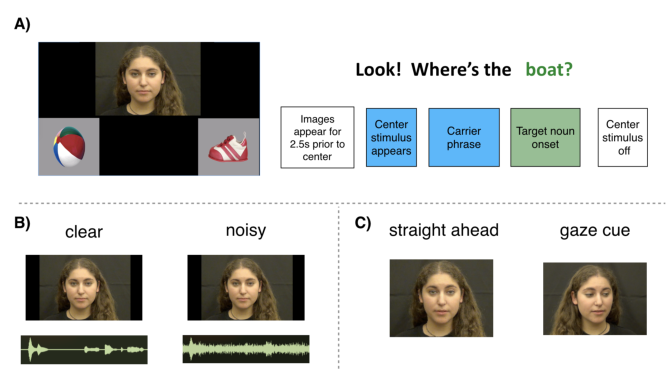
\includegraphics[width=0.9\linewidth]{figs/stimuli_plot-1} 

}

\caption[Stimuli for E1 and E2]{Stimuli for E1 and E2. Panel A shows the layout of the three fixation locations (speaker, target, and distracter), and the timecourse of a single trial. Panel B shows a visual representation of the clear and noisy waveforms used in E1. Panel C shows the social cue manipulation used in E2.}\label{fig:stimuli_plot}
\end{figure}
\end{CodeChunk}

\begin{CodeChunk}
\begin{figure*}[t]

{\centering 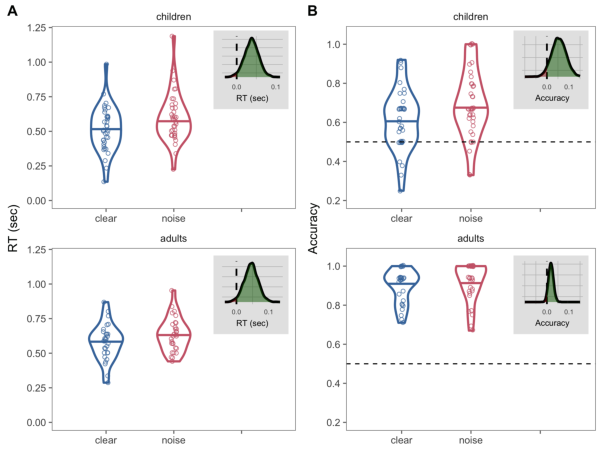
\includegraphics[width=0.8\linewidth]{figs/noise_acc_rt_e1_plot-1} 

}

\caption[Behavioral results from E1]{Behavioral results from E1. Panel A shows violin plots representing the distribution of median RTs for each participant in each condition. The dark red points represent the most likely estimate of the group mean with the error bars showing the 95\% Highest Density Interval. The grey inset plot shows the full posterior distribution of plausible RT differences across conditions with the vertical dashed line representing the null value of zero condition difference. The green shading represents estimates above the null value and the red shading represents estimates below the null value. Panel B shows the same information but for First Shift Accuracy.}\label{fig:noise_acc_rt_e1_plot}
\end{figure*}
\end{CodeChunk}

\subsection{Method}\label{method}

\subsubsection{Participants}\label{participants}

Participants were native, monolingual English-learning children (\(n=\)
39; 22 F, 17 M) and adults (\(n=\) 31; 22 F, 9 M). All participants had
no reported history of developmental or language delay and normal
vision. 14 participants (11 children, 3 adults) were run but not
included in the analysis because either the eye tracker falied to
calibrate or the participant did not complete the task.

\subsubsection{Stimuli}\label{stimuli}

\emph{Linguistic stimuli.} The stimuli were recorded in a sound-proof
room and featured two female speakers who used natural child-directed
speech and said one of two phrases: ``Hey! Can you find the (target
word)''" or ``Look! Where's the (target word) -- see panel A of Fig 1.
The target words were: ball, bunny, boat, bottle, cookie, juice,
chicken, and shoe. The target words varied in length (shortest = 411.68
ms, longest = 779.62 ms) with an average length of 586.71 ms.

\emph{Noise manipulation}. To create the noisy stimuli, we convolved the
recordings with Brown noise using the Audacity audio editor. The average
signal-to-noise ratio\footnote{The ratio of signal power to the noise
  power, with values greater than 0 dB indicating more signal than
  noise.} in the noise condition was 2.87 dB compared to the clear
condition, which was 35.05 dB.

\emph{Visual stimuli.} The image set consisted of colorful digitized
pictures of objects presented in fixed pairs with no phonological
overlap between the target and the distracter image (cookie-bottle,
boat-juice, bunny-chicken, shoe-ball). Side of target picture was
counterbalanced across trials.

\subsubsection{Design and procedure}\label{design-and-procedure}

Participants viewed the task on a screen while their gaze was tracked
using an SMI RED corneal-reflection eye-tracker mounted on an LCD
monitor, sampling at 60 Hz. The eye-tracker was first calibrated for
each participant using a 6-point calibration. On each trial,
participants saw two images of familiar objects on the screen for two
seconds before the center stimulus appeared (see Fig 1). Then they
processed the target sentence -- which consisted of a carrier phrase, a
target noun, and a question -- followed by two seconds without language
to allow for a response. Child participants saw 32 trials (16 noise
trials; 16 clear trials) with several filler trials interspersed to
maintain interest. Adult participants saw 64 trials (32 noise; 32
clear).

\subsection{Results and Discussion}\label{results-and-discussion}

\subsubsection{Analysis plan}\label{analysis-plan}

First, we present behavioral analyses of First Shift Accuracy and
Reaction Time (RT). RT corresponds to the latency to shift away from the
central stimulus to either picture measured from onset of the target
noun in the linguistic stimuli (we log transformed all RTs prior to
analysis). Accuracy corresponds to whether the participant's first gaze
shift landed on the target or the distracter picture. We used the
\texttt{rstanarm} (Gabry \& Goodrich, 2016) package to fit Bayesian
mixed-effects regression models. The mixed-effects approach allowed us
to model the nested structure in our data (multiple trials for each
participant; and a within-participants manipulation) by including random
intercepts for each participant and item, and a random slope for each
item and noise condition. We used Bayesian estimation to quantify the
uncertainty in our point estimates of the group means and condition
differences. To communicate this uncertainty we report the 95\% Highest
Density Interval (HDI), which provides a range of credible values given
the data and model. All analysis code can be found in the online
repository for this project:
\url{https://github.com/kemacdonald/speed-acc/R/analysis}.

Next, we present the two model-based analyses -- the EWMA and HDDM --
discussed in the introduction. Again, the goal of these models is to
move beyond a description of the data and map behavioral differences in
eye movements to underlying psychological variables. First, we use an
EWMA method to model changes in random shifting behavior as a function
of delays in responding (i.e., RT). For each RT, the model generates two
values: a ``control statistic'' (\textbf{CS}, which captures the running
average accuracy of first shifts) and an ``upper control limit''
(\textbf{UCL}, which captures the pre-defined threshold when gaze shifts
would be categorized as deviating from random responding). Here, the CS
is an expectation of random shifting to either the target or the
distracter image (nonlanguage-driven shifts), modeled a Bernoulli
process with \(P(success) = 0.5\). As participants delay their response,
we assume that they have gathered more information and should become
more accurate, which we model a Bernoulli process with
\(P(success) > 0.5\). Using this model, we can quantify and compare: a)
the cutoff point when the CS exceeds the UCL in the RT distribution,
indicating the processing time required before participants generated
language-driven shifts and b) the proportion of all gaze shifts that the
model categorizes as language-driven vs.~nonlanguage-driven.

Finally, we took the shifts that were categorized as language-driven by
the EWMA and fit a hierarchical Bayesian drift-diffusion model (HDDM) to
quantify differences in the underlying decision process that led to
different patterns of behavior. We chose to implement a hierarchical
Bayesian version of the DDM using the HDDM Python package (Wiecki,
Sofer, \& Frank, 2013) since we had relatively few trials from the child
participants and recent simulation studies have shown that the HDDM
approach was better than other DDM fitting methods for small data sets
(Ratcliff \& Childers, 2015). The model assumes that people accumulate
noisy evidence in favor of one alternative with a response generated
when the evidence crosses a pre-defined decision threshold. Here, we
focus on two parameters of interest that map onto meaningful decision
variables that we hypothesized would vary across our conditions:
\textbf{boundary separation}, which indexes the amount of evidence
gathered before generating a response (higher values suggest more
cautious responding) and \textbf{drift rate}, which indexes the amount
of evidence accumulated per unit time (higher values suggest more
efficient processing of the stimulus).

\subsubsection{Behavioral analyses}\label{behavioral-analyses}

\textbf{RT.} To make RTs more suitable for modeling on a linear scale,
we analyzed responses in log space using a logistic transformation, with
the final model was specified as:
\texttt{$log(RT) \sim noise\_condition + age\_group + (sub\_id + noise\_condition \mid item)$}.
Panel A of Figure 2 shows the full RT data distribution, the estimates
of condition means, and the full posterior distribution of the estimated
difference between the noise and clear conditions. Both children and
adults were slower to identify the target in the noise condition
(Children \(M_{noise}\) = 0.5 ms; Adult \(M_{noise}\) = 0.6 ms), as
compared to the clear condition (Children \(M_{clear}\) = 0.46 ms; Adult
\(M_{clear}\) = 0.55 ms). RTs in the noise condition were 42.55 ms
slower on average, with a 95\% HDI from 4.88 ms to 83.34 ms that did not
include the null value of zero condition difference.

\textbf{Accuracy.} Next, we modeled adults' and children's first shift
accuracy using a mixed-effects logistic regression with the same
specifications (see Panel B of Fig 2). Overall, both groups responded at
rates different from a model of random behavior (null value of \(0.5\)
falling well outside the lower bound of all group means). Adults were
more accurate (\(M_{adults} =\) 91\%) compared to children
(\(M_{adults} =\) 62\%). Both groups tended to be more accurate in
shifting to the target image in the noise condition (Children
\(M_{noise}\) = 67\%; Adult \(M_{noise}\) = 92\%) as compared to the
clear condition (Children \(M_{clear}\) = 62\%; Adult \(M_{clear}\) =
91\%). Accuracy in the noise condition was 4\% higher on average, with a
95\% HDI from 0\% to 11\%.Note that while the null value of zero
difference falls within the 95\% HDI, 96\% of the credible values fall
below the null, providing evidence for higher accuracy in the more
challenging noise condition.

\subsubsection{Model-based analyses}\label{model-based-analyses}

\begin{table}[b]
\centering
\begin{tabular}{lllr}
  \hline
Experiment & Parameter & Contrast & Estimate (95\% HDI) \\ 
  \hline
E1 & Cut point & age group & 0.21 [0.19, 0.24] \\ 
  E1 & Cut point & noise & 0.04 [0.01, 0.06] \\ 
  E1 & Guessing & age group & -0.46 [-0.49, -0.43] \\ 
  E1 & Guessing & noise & 0.12 [0.07, 0.17] \\ 
   \hline
E2 & Cut point & age group & 0.09 [0.03, 0.14] \\ 
  E2 & Cut point & gaze & 0 [-0.06, 0.06] \\ 
  E2 & Guessing & age group & -0.45 [-0.48, -0.42] \\ 
  E2 & Guessing & gaze & -0.03 [-0.07, 0] \\ 
   \hline
\end{tabular}
\caption{EWMA results for E1 and E2. Cut point refers to the response time in the RT distribution when gaze shifts reliably deviated from random. Guessing refers to the proportion of gaze shifts categorized as random vs. language-driven. Estimate refers to the average difference between condition or age group.} 
\end{table}

\textbf{EWMA.} Table 1 shows the interval of credible parameter
estiamtes for the age and condition contrasts in the EWMA model. Adults
started to produce accurate, language-driven shifts earlier in the RT
distribution (indexed by the lower cut point estimate) and a higher
proportion of language-driven responses overall (indexed by the lower
guessing parameter estimate). Critically, processing speech in noise
caused both adults and children to generate language-driven shifts later
in the RT distribution and produce a higher proprotion of
language-driven shifts. This pattern of results suggests that the noise
condition led participants to increase visual attention to the language
source, leading them to generate less exploratory, random shifting
behavior.

\textbf{HDDM.} Figure 3 shows the mean and the 95\% HDI of the posterior
distributions for the drift rate and boundary separation parameters.
Children had lower drift rates and boundary estimates as compared to
adults, suggesting that children were less efficient and less cautious
in their responding. Critically, the noise manipulation modulated the
boundary separation parameter, with higher estimates in the noisy
processing context for both age groups. This pattern of model output
suggests that the higher levels of accuracy in the noise condition were
driven by listeners accumulating more evidence before generating an eye
movement, as opposed to processing the information with differential
efficiency.

\begin{CodeChunk}
\begin{figure}[t]

{\centering 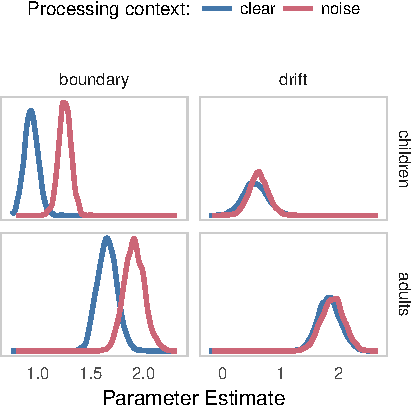
\includegraphics[width=0.85\linewidth]{figs/hddm_plot_noise-1} 

}

\caption[HDDM results E1]{HDDM results E1.}\label{fig:hddm_plot_noise}
\end{figure}
\end{CodeChunk}

Taken together, the behavioral analyses and the EWMA/HDDM results
provide converging support that processing speech in noise caused
listeners to seek additional visual information to support language
comprehension. Interestingly, we saw a strikingly similar pattern of
results in children and adults, with both groups producing more
language-driven shifts and prioritizing accuracy over speed in the
noisier processing context. The adaptive response in our task has
interesting parallels to recent work by McMurray, Farris-Trimble, \&
Rigler (2017), showing that adults with Cochlear Implants, who must deal
with degraded auditory input, will delay the process of lexical acesss,
waiting to begin until substantial information has accumulated. This is
in contrast to an ``immediate competion'' model of word recognition
where candidate meanings are activated from the onset of the word.

Degrading the auditory signal is one way to make the visual information
more useful. However, there are many ecologically valid processing
contexts where aspects of the visual world provide particularly useful
information. In E2, we set out to test our account in one of these
contexts: processing speech accompanied by a visual cue to reference, a
speaker's eye gaze.

\begin{CodeChunk}
\begin{figure*}[tb]

{\centering 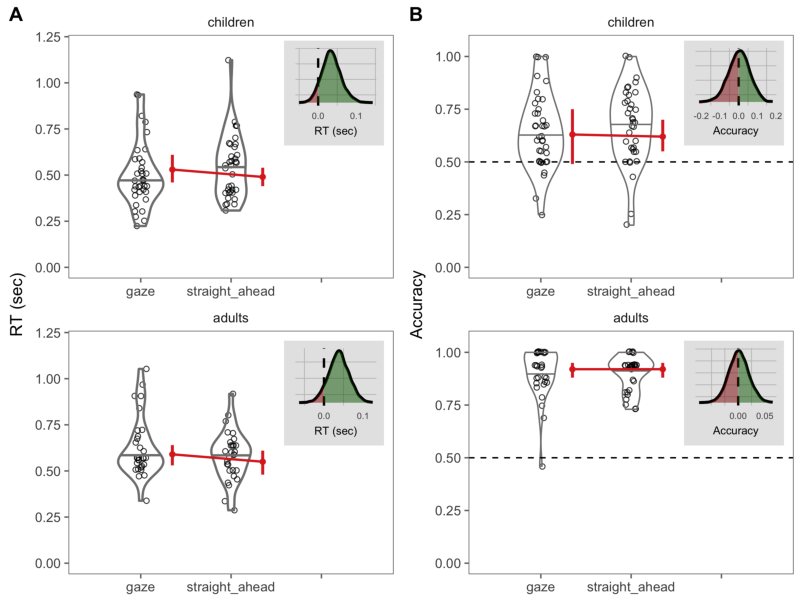
\includegraphics[width=0.8\linewidth]{figs/gaze_acc_rt_e2_plot-1} 

}

\caption[Behavioral results from E2]{Behavioral results from E2. All plotting conventions are the same as in Figure 2.}\label{fig:gaze_acc_rt_e2_plot}
\end{figure*}
\end{CodeChunk}

\section{Experiment 2}\label{experiment-2}

In E2, we ask whether increasing the information value of the speaker as
a fixation target will produce a similar speed-accuracy tradeoff effect
as we saw in E1. We compared the timing of eye movements to disegnage
from a language source across two processing contexts: speech with and
without a social cue to reference (a speaker's gaze). We hypothesized
that the gaze cue would cause listeners to delay shifting gaze to
accumulate more information, leading to more accurate deicisions. Our
key behavioral prediction was that participants in the Gaze conditions
should produce a higher proportion of language-driven shifts as indexed
by the EWMA model output and higher boundary parameter estimates in the
DDM model.

\subsection{Method}\label{method-1}

\subsubsection{Participants}\label{participants-1}

Participants were native, monolingual English-learning children (\(n=\)
38; 19 F, 19 M) and adults (\(n=\) 31; 22 F, 9 M). All participants had
no reported history of developmental or language delay and normal
vision. 12 participants (9 children, 3 adults) were run but not included
in the analysis either because the eye tracker falied to calibrate or
the participant did not complete the task.

\subsubsection{Stimuli}\label{stimuli-1}

The audio stimuli were identical to the clear stimuli used in E1. We
included a new center fixation stimulus type: a vidoe with a
post-nominal gaze cue (see Fig 1). The onset of gaze occurred at the end
of each target noun. We chose a post-nominal cue to give us the best
opportunity to detect whether participants would delay shifting away
from the speaker to gather the additional visual information prior to
seeking the named referent.

\subsubsection{Design and procedure}\label{design-and-procedure-1}

The design was identical to E1. Child participants saw 32 trials (16
gaze trials; 16 straight ahead trials) with several filler trials
interspersed to maintain interest. Adult participants saw 64 trials (32
gaze; 32 straight ahead). The gaze manipulation was presented in a
blocked design with order of block counterbalanced across participants.

\subsection{Results and Discussion}\label{results-and-discussion-1}

\subsubsection{Behavioral analyses}\label{behavioral-analyses-1}

\textbf{RT.} Panel A of Figure 4 shows the full RT data distribution,
the estimates of condition means, and the full posterior distribution of
the estimated difference between the gaze and straight-ahead conditions.
Both age groups responed with similar speed and accuracy. The average
difference in RTs in the gaze condition was 36.32 ms, with a 95\% HDI
from -13.16 ms to 89.03 ms that did included the null value of zero
condition difference.

\textbf{Accuracy.} Next, we quantified adults' and children's first
shift accuracy. Overall, both groups were more accurate than a model of
random behavior (null value of \(0.5\) falling well outside the lower
bound of all group means). Adults were more accurate (\(M_{adults} =\)
91\%) compared to children (\(M_{adults} =\) 62\%). And both groups were
equally accurate across the gaze conditions with the average difference
being 0\%, with a 95\% HDI from -9\% to 9\% that incluced the null value
of zero condition difference.

\subsubsection{Model-based analyses}\label{model-based-analyses-1}

\textbf{EWMA.} Table 1 shows the interval of credible parameter
estiamtes for the age and condition contrasts in the EWMA model. Similar
to E1, adults started to produce accurate, language-driven shifts
earlier in the RT distribution and generated a higher proportion of
language-driven responses compared to children. There was some evidence
that the presence of gaze increased the proportion of language-driven
shifts, but not the cut point parameter. This pattern of results
suggests that the gaze condition led listeners to increase visual
attention to the language source, leading them to generate fewer early
random gaze shifts.

\textbf{HDDM.} Figure 4 shows the mean and the 95\% HDI of the posterior
distributions for the drift rate and boundary separation parameters.
Parallel to E1, children had lower drift rates and boundary estimates as
compared to adults. We saw high overlap in the posterior distributions
for both parameters across the two gaze contexts in children, but there
was some evidence that the presence of gaze increased boundary
separation and decreased drift for adults. This suggests that when we
analyzed ``language-driven'' shifts, we see evidence that adults
achieved comparable accuracy across condition, but accumulated more
information prior to responding when processing speech accompanied by
social cue to reference.

\begin{CodeChunk}
\begin{figure}[t]

{\centering 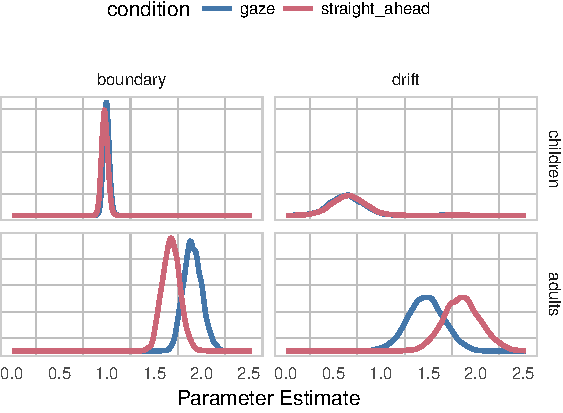
\includegraphics[width=0.85\linewidth]{figs/hddm_plot_gaze-1} 

}

\caption[HDDM results E2]{HDDM results E2.}\label{fig:hddm_plot_gaze}
\end{figure}
\end{CodeChunk}

\section{General Discussion}\label{general-discussion}

Language comprehension in grounded contexts involves integrating the
visual and linguistic signals. But the value of visual information can
vary depending on what information is available to the listener and the
quality of the incoming language. In this work, we tested two
predictions of an information-maximization account of eye movements
during language processing -- an account that we proposed in K.
MacDonald et al. (2017) to explain population-level differences between
the gaze dynamics of children learning ASL and children learning spoken
English. In E1, we showed that children and adults adapt to processing
speech in noise by producing slower but more accurate gaze shifts away
from a language source. Both groups also showed evidence of prioritizing
information accumulation over speed of responding, and they produced
more language driven shifts compared to processing speech in a clear
context. This adaptive response is striking since listeners compensated
such that they more accurate in the more challenging context. In E2, we
saw some evidence -- more so for adults than for children -- that the
presence of a social cue to reference (eye gaze) caused listeners to
delay their responses and to generate more languge-driven shifts. These
results represent a confimatory test of the linguistic signal increases,
eye movements to the \emph{rest} of the visual world become less useful
and occur less often.

These results connect to ideas from several rich research programs and
theoretical accounts. First, research on language-mediated visual
attention shows that adults and children rapidly shift gaze upon hearing
the name of an object in the visual scene (Allopenna, Magnuson, \&
Tanenhaus, 1998; Tanenhaus, Spivey-Knowlton, Eberhard, \& Sedivy, 1995).
The speed and consistency of this behavior has led to debates about
whether language-mediated gaze shifts are automatic as opposed to under
the control of the listener. While we do not think that listeners in our
task have explicit access to the underlying shift, our findings show
that the dynamics of gaze during lexical can access adapt to the
information features of the processing context. This finding parallels
recent work by McMurray et al. (2017), showing that adults with Cochlear
Implants, who consistently process degraded auditory input, will delay
the process of lexical acesss, waiting to begin until substantial
information has accumulated.

Second, empirical work on vision during natural tasks shows that people
overwhelmingly prefer to look at \emph{goal-relevant} locations -- e.g.,
an upcoming obstacle while walking (Hayhoe \& Ballard, 2005). These
accounts inspired our prediction that gaze dynamics during language
comprehension should adapt to the value of different fixation behaviors
with respect to the listener's goal of rapid language processing. And
third, work on effortful listening shows that listeners generate
compensatory responses (e.g., increases in attention and working memory)
within ``challenging'' comprehension contexts such as processing noisy
or accented speech (Van Engen \& Peelle, 2014). These accounts predict
that our young listeners might compensate for the reduced quality of the
auditory signal by allocating gathering additional visual information.

This work has several important limitations that we hope will pave the
way for future work. Here, we chose to focus on a single decision about
visual fixation to provide a window onto the underlying dynamics of
decision-making across different processing contexts. However, the
decision to shift away from a language is just one of the \emph{many}
decisions that listeners make while processing language in real-time.
Moreover, our micro-analysis does not consider the rich gaze patterns
that occur prior to this decision. In our future work, we aim to
quantify changes in the dynamics of gaze across the full sentence
processing context. Finally, we used a very simple visual world, with
only three places to look, and very simple linguistic stimuli,
especially for the adults. Thus it remains an open question how these
results might scale up to more complex language information and visual
environments.

We designed these experiments to test our information-maximization
proposal in the domain of familiar language comprehension. However, we
think the account is more general. And we are interested in applying
this framework -- the use of in-depth analyses of the micro-level
decisions about visual fixation -- to the early language
\emph{acquisition} context. Consider that early in language learning
children are acquiring novel word-object links while also learning about
visual object categories. Both of these tasks produce goals that should
shape children's decisions about visual fixation, e.g., changing the
information value of looks to a speaker vs.~looks to an object. More
generally, we think that these results contribute to recent theoretical
work emphasizing the need for goal-based accounts of eye movements
during language comprehension (Salverda, Brown, \& Tanenhaus, 2011). And
we hope that our approach offers a way forward to explain fixation
behaviors across a wider variety of populations, processing contexts,
and during different stages of language learning.

\section{Acknowledgements}\label{acknowledgements}

We are grateful to the families who participated in this research.
Thanks to Tami Alade and Hannah Slater for help with data collection.
This work was supported by an NSF GRFP to KM.

\section{References}\label{references}

\setlength{\parindent}{-0.1in} \setlength{\leftskip}{0.125in} \noindent

\hypertarget{refs}{}
\hypertarget{ref-allopenna1998tracking}{}
Allopenna, P. D., Magnuson, J. S., \& Tanenhaus, M. K. (1998). Tracking
the time course of spoken word recognition using eye movements: Evidence
for continuous mapping models. \emph{Journal of Memory and Language},
\emph{38}(4), 419--439.

\hypertarget{ref-brooks2008infant}{}
Brooks, R., \& Meltzoff, A. N. (2008). Infant gaze following and
pointing predict accelerated vocabulary growth through two years of age:
A longitudinal, growth curve modeling study. \emph{Journal of Child
Language}, \emph{35}(01), 207--220.

\hypertarget{ref-clark2009first}{}
Clark, E. V. (2009). \emph{First language acquisition}. Cambridge
University Press.

\hypertarget{ref-erber1969interaction}{}
Erber, N. P. (1969). Interaction of audition and vision in the
recognition of oral speech stimuli. \emph{Journal of Speech and Hearing
Research}, \emph{12}(2), 423--425.

\hypertarget{ref-gabry2016rstanarm}{}
Gabry, J., \& Goodrich, B. (2016). Rstanarm: Bayesian applied regression
modeling via stan. r package version 2.10. 0.

\hypertarget{ref-hayhoe2005eye}{}
Hayhoe, M., \& Ballard, D. (2005). Eye movements in natural behavior.
\emph{Trends in Cognitive Sciences}, \emph{9}(4), 188--194.

\hypertarget{ref-macdonald1978visual}{}
MacDonald, J., \& McGurk, H. (1978). Visual influences on speech
perception processes. \emph{Attention, Perception, \& Psychophysics},
\emph{24}(3), 253--257.

\hypertarget{ref-macdonald2017info}{}
MacDonald, K., Blonder, A., Marchman, V. and, Fernald, A., \& Frank, M.
C. (2017). An information-seeking account of eye movements during spoken
and signed language comprehension. In \emph{Proceedings of the 39th
annual conference of the cognitive science society}.

\hypertarget{ref-macdonald2006constraint}{}
MacDonald, M. C., \& Seidenberg, M. S. (2006). Constraint satisfaction
accounts of lexical and sentence comprehension. \emph{Handbook of
Psycholinguistics}, \emph{2}, 581--611.

\hypertarget{ref-mcclelland2006there}{}
McClelland, J. L., Mirman, D., \& Holt, L. L. (2006). Are there
interactive processes in speech perception? \emph{Trends in Cognitive
Sciences}, \emph{10}(8), 363--369.

\hypertarget{ref-mcmurray2017waiting}{}
McMurray, B., Farris-Trimble, A., \& Rigler, H. (2017). Waiting for
lexical access: Cochlear implants or severely degraded input lead
listeners to process speech less incrementally. \emph{Cognition},
\emph{169}, 147--164.

\hypertarget{ref-ratcliff2015individual}{}
Ratcliff, R., \& Childers, R. (2015). Individual differences and fitting
methods for the two-choice diffusion model of decision making.
\emph{Decision}, \emph{2}(4), 237--279.

\hypertarget{ref-salverda2011goal}{}
Salverda, A. P., Brown, M., \& Tanenhaus, M. K. (2011). A goal-based
perspective on eye movements in visual world studies. \emph{Acta
Psychologica}, \emph{137}(2), 172--180.

\hypertarget{ref-smith2017multimodal}{}
Smith, A. C., Monaghan, P., \& Huettig, F. (2017). The multimodal nature
of spoken word processing in the visual world: Testing the predictions
of alternative models of multimodal integration. \emph{Journal of Memory
and Language}, \emph{93}, 276--303.

\hypertarget{ref-tanenhaus1995integration}{}
Tanenhaus, M. K., Spivey-Knowlton, M. J., Eberhard, K. M., \& Sedivy, J.
C. (1995). Integration of visual and linguistic information in spoken
language comprehension. \emph{Science}, \emph{268}(5217), 1632.

\hypertarget{ref-van2014listening}{}
Van Engen, K. J., \& Peelle, J. E. (2014). Listening effort and accented
speech. \emph{Frontiers in Human Neuroscience}, \emph{8}.

\hypertarget{ref-vandekerckhove2007fitting}{}
Vandekerckhove, J., \& Tuerlinckx, F. (2007). Fitting the ratcliff
diffusion model to experimental data. \emph{Psychonomic Bulletin \&
Review}, \emph{14}(6), 1011--1026.

\hypertarget{ref-wiecki2013hddm}{}
Wiecki, T. V., Sofer, I., \& Frank, M. J. (2013). HDDM: Hierarchical
bayesian estimation of the drift-diffusion model in python.
\emph{Frontiers in Neuroinformatics}, \emph{7}, 14.

\end{document}
